\chapter{QMapIterator}

template <typename Key, typename T> class QMapIterator

QMapIterator 类为 QMap 和 QMultiMap 提供 Java 风格的常量迭代器。更多内容...

\begin{tabular}{|r|l|}
	\hline
	属性 & 方法 \\
	\hline
	头文件 & \#include <QMapIterator>\\      
	\hline
	qmake & QT += core\\      
	\hline
\end{tabular}

\begin{compactitem}
\item 所有成员列表,包括继承的成员
\end{compactitem}

\section{公共成员函数}

\begin{longtable}{|r|l|}
\hline
& QMapIterator(const QMap<Key, T> \&map) \\ 
\hline
QMapIterator<Key, T> \& 	& operator=(const QMap<Key, T> \&container) \\ 
\hline
bool 	& findNext(const T \&value) \\ 
\hline
bool 	& findPrevious(const T \&value) \\
\hline
bool &	hasNext() const \\
\hline
bool &	hasPrevious() const \\ 
\hline
const Key & 	key() const \\
\hline
QMapIterator::Item &	next() \\ 
\hline
QMapIterator::Item 	&peekNext() const \\ 
\hline
QMapIterator::Item &	peekPrevious() const \\ 
\hline
QMapIterator::Item 	&previous() \\ 
\hline
void 	&toBack() \\
\hline
void 	&toFront() \\ 
\hline
const T \& & 	value() const \\ 
\hline
\end{longtable}

\section{详细描述}

QMap 同时提供 Java 风格迭代器 和 STL 风格迭代器。
Java 风格迭代器比 STL 风格迭代器更高级,更容易使用;
同时也略微低效。

QMapIterator<Key, T> 用来遍历 QMap (或 QMultiMap)。
如果想在遍历时修改 map,要使用 QMutableMapIterator。

QMapIterator 构造函数接受 QMap 作为参数。
构造后,迭代器位于 map 的最开始位置(第一个元素之前)。
下面的例子演示如何顺序遍历所有元素:

\begin{lstlisting}[language=C++]
QMap<int, QWidget *> map;
...
QMapIterator<int, QWidget *> i(map);
while (i.hasNext()) {
    i.next();
    qDebug() << i.key() << ": " << i.value();
}
\end{lstlisting}

next() 函数返回 map 中的下一个元素并将迭代器前移。
key() 和 value() 函数返回跳过的最后一个元素的键和值。

与 STL 风格迭代器不同,Java 风格迭代器指向元素之间而不是直接指向元素。
第一次调用 next() 前移迭代器到第一个和第二个元素之间的位置,并返回第一个元素;
第二次调用 next() 前移迭代器到第二个和第三个元素之间的位置;以此类推。


\begin{figure}[hpt!]  
	\centering
    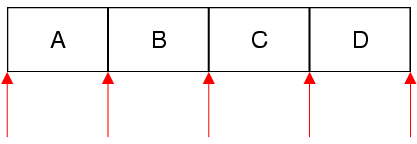
\includegraphics[width=0.5\textwidth]{javaiterators1}
\end{figure}

%%%%%%%%

下面的例子演示如何反序遍历元素:

\begin{lstlisting}[language=C++]
QMapIterator<int, QWidget *> i(map);
i.toBack();
while (i.hasPrevious()) {
    i.previous();
    qDebug() << i.key() << ": " << i.value();
\end{lstlisting}

如果想查找特定值的所有实例,循环使用 findNext() 或 findPrevious()。例如:

\begin{lstlisting}[language=C++]
QMapIterator<int, QWidget *> i(map);
while (i.findNext(widget)) {
    qDebug() << "Found widget " << widget << " under key "
             << i.key();
}
\end{lstlisting}

同一 map 可以使用多个迭代器。
如果在 QMapIterator 处于活动状态时修改 map,QMapIterator 将继续在原 map 上遍历,
而忽略修改后的副本。

\begin{seeAlso}
QMutableMapIterator 和 QMap::const\_iterator。
\end{seeAlso}

\section{成员函数文档}

bool QMapIterator::findPrevious(const T \emph{\&value})

从当前迭代器位置开始向后查找值 \emph{value}。
如果找到值为 \emph{value} 的键值对,返回 true;
否则返回 false。

调用该函数后,如果找到值,迭代器将被移动到匹配元素的前面;
否则,迭代器将被移动到容器的前端。

\begin{seeAlso}
findNext()。
\end{seeAlso}

\splitLine

bool QMapIterator::findNext(const T \emph{\&value})

从当前迭代器位置开始向前查找值 \emph{value}。
如果找到值为 \emph{value} 的键值对,返回 true;
否则返回 false。

调用该函数后,如果找到值 \emph{value},迭代器将被移动到匹配元素的后面;
否则,迭代器将被移动到容器的末端。

\begin{seeAlso}
findPrevious()。
\end{seeAlso}
    
\splitLine

const Key \&QMapIterator::key() const

调用遍历函数(next(),previous(),findNext(),findPrevious())后,该函数返回跳过的最后一个元素的键。

调用 next() 或 findNext() 后,key() 与 peekPrevious().key() 相同。调用 previous() 或 findPrevious() 后,key() 与 peekNext().key() 相同。

\begin{seeAlso}
value()。
\end{seeAlso}

\splitLine

QMapIterator::Item QMapIterator::peekPrevious() const

不移动迭代器而返回前一个元素。

对返回值调用 key() 获取元素的键,调用 value() 获取元素的值。

对位于容器前端的迭代器调用该函数将导致未定义结果。

\begin{seeAlso}
hasPrevious(),previous() 和 peekNext()。
\end{seeAlso}

\splitLine

QMapIterator::Item QMapIterator::previous()

返回前一个元素并将迭代器向后移动一个位置。

对返回值调用 key() 获取元素的键,调用 value() 获取元素的值。

对位于容器前端的迭代器调用该函数将导致未定义结果。


\begin{seeAlso}
hasPrevious(),peekPrevious() 和 next()。
\end{seeAlso}

\splitLine

bool QMapIterator::hasPrevious() const

如果该迭代器前面至少有一个元素,返回 true,即该迭代器不在容器的前端;否则返回 false。

\begin{seeAlso}
hasNext() 和 previous()。
\end{seeAlso}

\splitLine

bool QMapIterator::hasNext() const

如果该迭代器后面至少有一个元素,返回 true,即该迭代器不在容器的末端;否则返回 false。

\begin{seeAlso}
hasPrevious() 和 next()。
\end{seeAlso}

\splitLine

void QMapIterator::toBack()

将迭代器移动到容器的末端(最后一个元素之后)。

\begin{seeAlso}
toFront() 和 previous()。
\end{seeAlso}

\splitLine

void QMapIterator::toFront()

将迭代器移动到容器的前端(第一个元素之前)。

\begin{seeAlso}
toBack() 和 next()。
\end{seeAlso}

\splitLine

QMapIterator<Key, T> \&QMapIterator::operator=(const QMap<Key, T> \emph{\&container})

将迭代器关联到 \emph{container} 来遍历 map。迭代器将被移动到 map 的前端(第一个元素之前)。


\begin{seeAlso}
toFront() 和 toBack()。
\end{seeAlso}

\splitLine

QMapIterator::QMapIterator(const QMap<Key, T> \emph{\&map})

构造一个迭代器来遍历 \emph{map}。迭代器将被移动到 \emph{map} 的前端(第一个元素之前)。


\begin{seeAlso}
operator=()。
\end{seeAlso}

\splitLine

QMapIterator::Item QMapIterator::next()

返回下一个元素并将迭代器向前移动一个位置。

对返回值调用 key() 获取元素的键,调用 value() 获取元素的值。

对位于容器末端的迭代器调用该函数将导致未定义结果。

\begin{seeAlso}
hasNext(),peekNext() 和 previous()。
\end{seeAlso}
    
\splitLine

QMapIterator::Item QMapIterator::peekNext() const

不移动迭代器而返回下一个元素。

对返回值调用 key() 获取元素的键,调用 value() 获取元素的值。

对位于容器末端的迭代器调用该函数将导致未定义结果。

\begin{seeAlso}
hasNext(),next() 和 peekPrevious()。
\end{seeAlso}

\splitLine

const T \&QMapIterator::value() const

调用遍历函数(next(),previous(),findNext(),findPrevious())后,该函数返回跳过的最后一个元素的值。

调用 next() 或 findNext() 后,value() 与 peekPrevious().value() 相同。

调用 previous() 或 findPrevious() 后,value() 与 peekNext().value() 相同。

\begin{seeAlso}
key()。
\end{seeAlso}